% Chapter 6
\chapter{Advertisement High Fidelity prototype} % Main chapter title

\label{Chapter6} % For referencing the chapter elsewhere, use \ref{Chapter1} 

\newpage

\section{Introduction}
A follow up study is conducted when a final version of a prototype is developed, this is called \emph{summative study}, \cite{summative} ``\emph{it is used to evaluate how well the design meets the usability requirements}'' it is to make some final decisions on the prototype, there have been studies like ``\emph{Sweep and point \& shoot}'' \cite{SweepPointShoot} that evaluated prototypes of interaction of personal computing device with large public displays, another was an evaluation of ``\emph{mobile interaction with live video}'' \cite{TouchProjector}, which was a with-in subject design, the participant’s performance were measured for automatic zooming and temporary image freezing. Sebastian .D \cite{WalldragandDrop} assessed the general performance of drag and drop interaction on large displays and compared it with a traditional drag and drop. Jorg Müller \cite{LookingGlass} did pre-studies (lab and field) on noticing interactivity of a display in which the time required for recognizing interactivity by participants were measured.

Based on the feedbacks from the low-fidelity evaluation in previous chpater, I developed the hi-fidelity version of interactive advertisement both (body, mobile), which was at a functional level. This chapter explains the evaluation process of Hi-fidelity prototypes of interactive advertisement both body and mobile. The evaluations were more on user performance, user acceptance; it also focused on the possible usability issues. As the application would be in public, where many people would interact, therefor this study also tested the application performance with single and multi-users to ensure application stability.



\section{Advertisement prototypes}
The prototype was to show a city map on the screen with possible interactive famous places of Bauhaus, the interaction idea was to map physical movement of the user, or map the cursor movement of a phone to the virtual movement on the city map, and let user to explore the target places by reaching to those locations. Three to five places were to be explored by one person to finish the interaction.


There are mainly three hierarchical levels of interfaces, (1) \emph{call-to-action}, (2) \emph{Game interaction}, and (3) the advertisement video interface.

\begin{itemize}
\item Call-to-Action interface: \\
This interface invites participants to interact with the application, this method was first proposed by Bill Kules \cite{call-to-action}, in which the immediate usability of public accesses to a system was designed. \emph{call-to-action} of body and mobile are designed differently, which are shown in below sections. 

\item Interaction interface: \\
This interface activates when the user follow the instructions of the first interface, the interface shows the interactive map with the hotspots to be explored by participants.
\item video advertisement: \\
After the interaction finishes then a silent video advertisement is shown for 20 seconds. 
The advertisement video was created in powtoon\footnote{Powtoon: \url{https://www.powtoon.com}, last accessed: 21 April 2016} with a free version account, to see the full advertisement video visit below link.\\ 
Old video version: \url{https://www.youtube.com/watch?v=GrWtOyjNcQ0}
New video version: \url{https://www.youtube.com/watch?v=-y1Dbz6E6bU&feature=youtu.be}
\end{itemize}


\newpage
\subsection{Body prototype}
This section introduces the interfaces of the body interactive prototypes and the processes that how a user can start interaction. \\
\hilight{make the video demo}


\begin{enumerate}

\item call-to-action interface: \\

This interface is basically the attraction attention and call-to-action interface, as you can see below there is someone standing in front of the screen and the interface calls him to come near. This area also has alert message on the top right area of the screen and alerts the participant if they move away from the camera range, in this example the person is standing but there is also the second person but got immediately untracked and the system pops that message to raise his hand to be tracked again.

\begin{figure}[H]
    \centering
    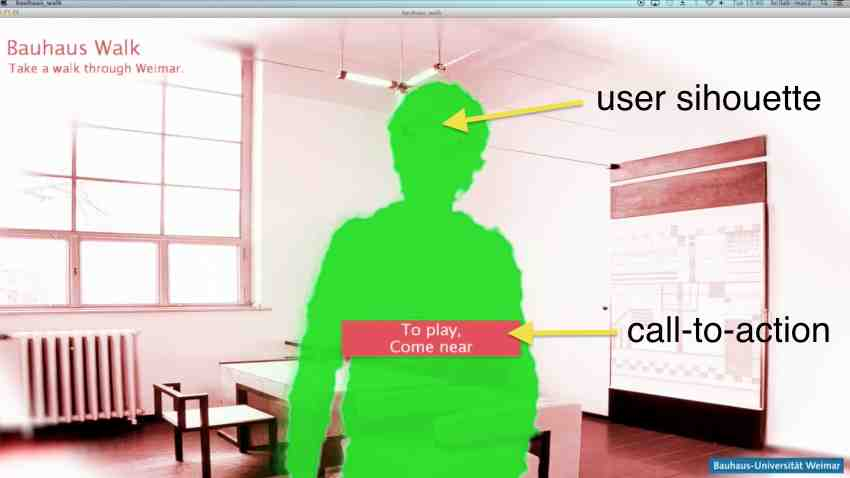
\includegraphics[width=120mm,height=70mm]{Figures/6/body/first_interface}
    \caption{call-to-action interface}%
    \label{fig:body_firstinterface}%
\end{figure}

When the person steps in the range of the Camera, his silhouette is projected on the screen with a different color, the application calls the person to come near in order to trigger the game.

\item Transition to interaction interfaces: \\
The transition happens when the person stands close to the screen for more than 3 seconds and the below things happen.

\begin{enumerate}
\item Loading animation:\\
  The loading animation is a reaction to the action of the participants, and at the same time participants waits for something to be loaded.
\item Scaling down the silhouette: \\
To walk freely on the map and to give the participant the feeling of walking, the participant's silhouette is scaled down, the scaling happens smoothly frame-by-frame.
\item Show task instruction:  \\
Every interaction has instructions, the instruction is fairly very easy and it is simplified in one sentence to explore locations on the map.
\end{enumerate}

\begin{figure}[H]
    \centering
    \begin{subfigure}[H]{0.3\textwidth}
        \centering
        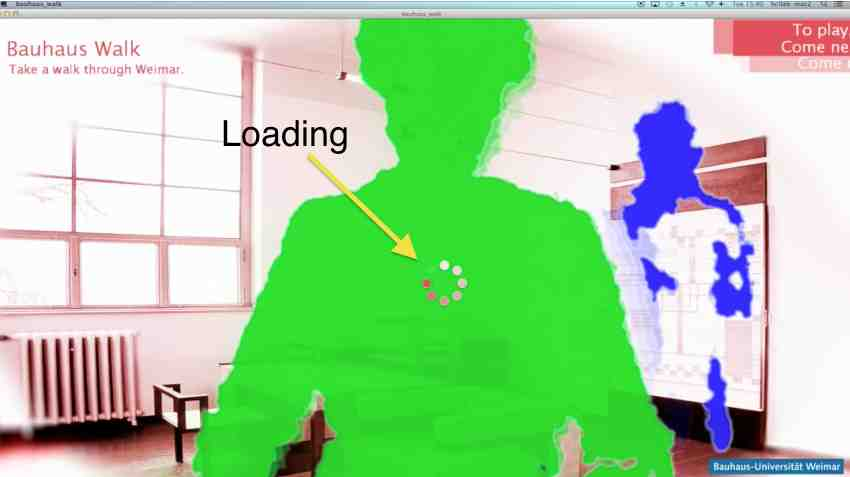
\includegraphics[width=\textwidth,height = 3.5cm]{Figures/6/body/loading}
        \caption{Loading}
        \label{fig:loading_logo}
    \end{subfigure}
    \begin{subfigure}[H]{0.3\textwidth}
        \centering
        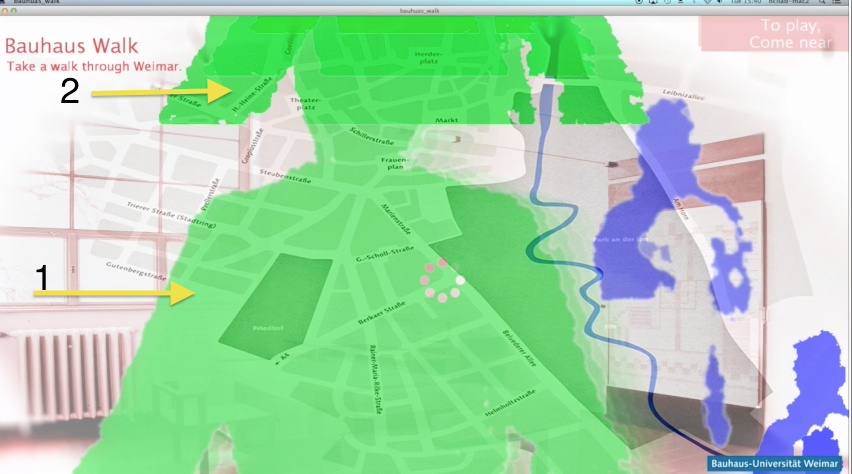
\includegraphics[width=\textwidth,height = 3.5cm]{Figures/6/body/scalling_down}
        \caption{Scalling down}
        \label{fig:scalling_down}
    \end{subfigure} 
      \begin{subfigure}[H]{0.3\textwidth}
        \centering
        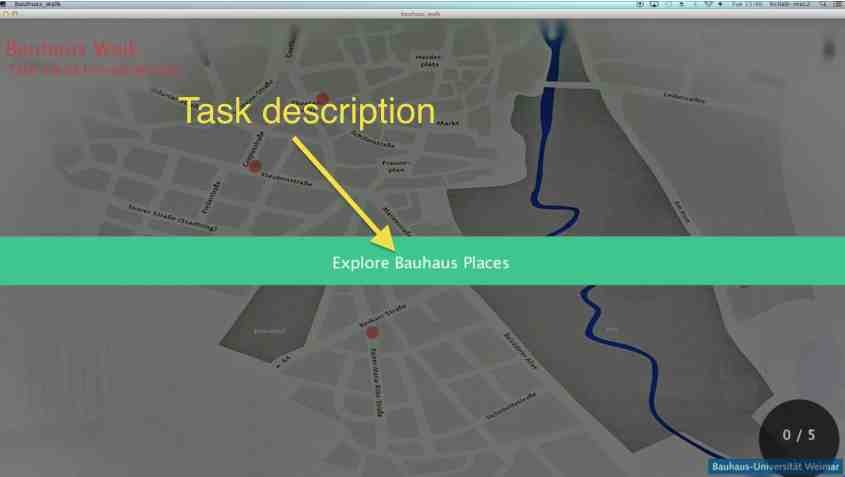
\includegraphics[width=\textwidth,height = 3.5cm]{Figures/6/body/task_description}
        \caption{Task description}
        \label{fig:task_description}
    \end{subfigure}
    \caption{Transitions of interfaces }
    \label{fig:transition_sequence}
\end{figure}


\item Interaction interface: \\
In this interface participants can interact with the elements on the map. As shown in picture below, the silhouette has visited four locations therefor has 4/5 score, to finish the interaction he needs to visit the last one location.

\begin{figure}[H]
    \centering
    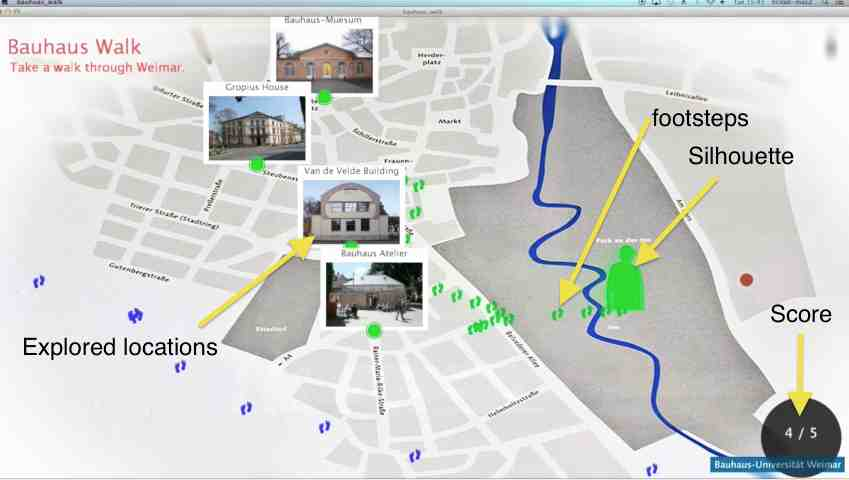
\includegraphics[width=130mm,height=80mm]{Figures/6/body/interaction_inter}
    \caption{Second Interface}%
    \label{fig:body_secondinterface}%
\end{figure}

%\subsubsection{Flowchart Diagram}
%The below chart roughly shows the flow of the application.
%\begin{figure}[H]
%    \centering
%    \includegraphics[width=120mm,height=140mm]{Figures/7/body_interactive/body_flow_chart}
%    \caption{Body Interactive advertisement Flowchart diagram}%
%    \label{fig:Body_flowchat}%
%\end{figure}

\end{enumerate}

\subsection{Mobile}
Mobile interaction is possible by using a smartphone and a Wi-Fi connection to the advertisement network, the user should open the mentioned IP address in his / her mobile browser and enter a name to login. 
\hilight{make the video demo}


\begin{enumerate}

\item call-to-action interface: \\
This interface is designed in such a way to attract passers-by and also guide the participant on how to use their smartphone to access the advertisement application. The attraction is again the same method that was used for body, the passers-by silhouette is projected at the back of Access information. The interface has QR code that could be easy to be scanned instead of typing the whole IP address, and there is an alert area, that gets activated when a logged in person has not turned their phone in landscape orientation.

\begin{figure}[H]
    \centering
    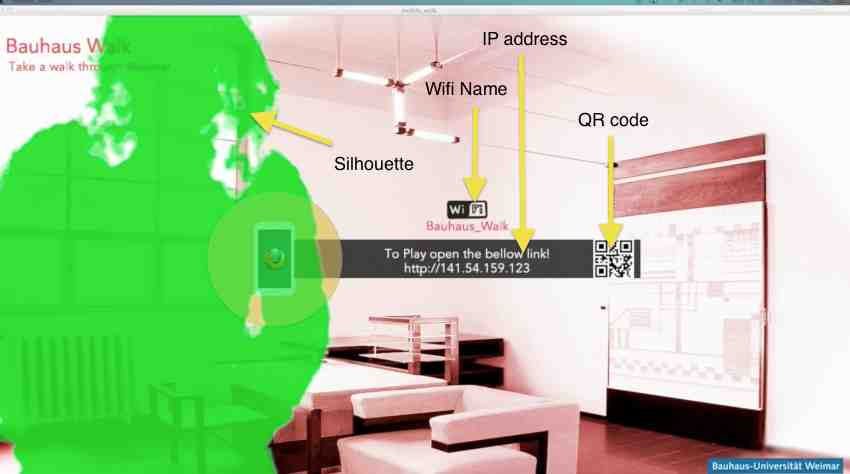
\includegraphics[width=120mm,height=70mm]{Figures/6/mobile/call-to-action}
    \caption{Mobile interactive interface:}%
    \label{fig:mobile_firstinterface}%
\end{figure}



\item Transition to interaction interfaces: \\
The transition happens only when the user connects to the Wifi, open the controller and physically hold the phone in landscape.

\begin{enumerate}
\item Loading animation:\\
  The loading animation is a reaction to the action of the participants, and at the same time participants waits for something to be loaded.
\item  Creating Colored cursor: \\
A colored circle will be created for the participant in the center of the screen; each participant would have different colors matching to their controller interface in their phone.
\item Show task instruction:  \\
The instruction is fairly very easy and it is simplified in one sentence to explore locations on the map by using their phone.

\end{enumerate}


\begin{figure}[H]
    \centering
    \begin{subfigure}[H]{0.45\textwidth}
        \centering
        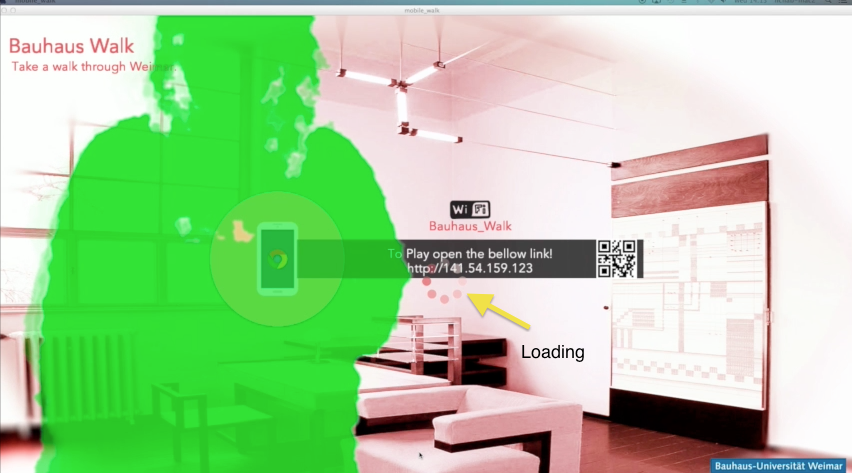
\includegraphics[width=\textwidth,height=4cm]{Figures/6/mobile/loading}
        \caption{Loading}
        \label{fig:loading_mobile}
    \end{subfigure}
    \begin{subfigure}[H]{0.45\textwidth}
        \centering
        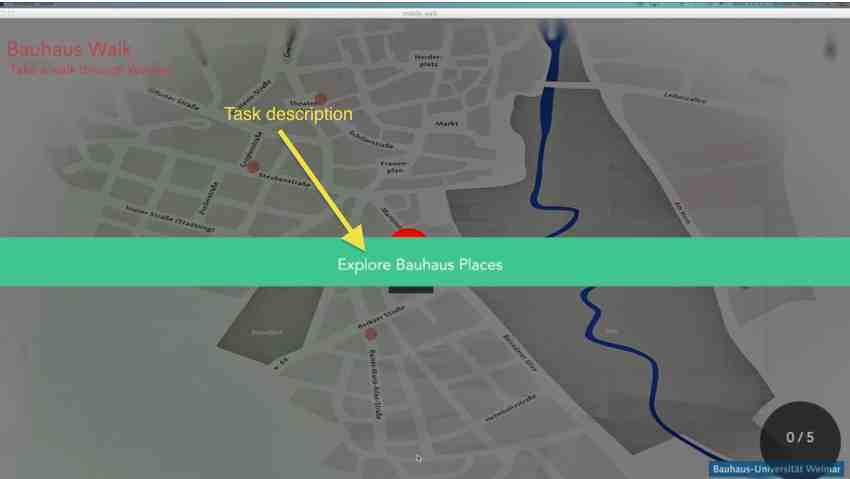
\includegraphics[width=\textwidth,height=4cm]{Figures/6/mobile/task_desc}
        \caption{Task description}
        \label{fig:task_mobile}
    \end{subfigure}
    \caption{Transitions of interfaces.}
    \label{fig:Switching_between_phases_mobile}
\end{figure}


\item Interation interface" \\
Second screen is the interaction screen for the participants, participants can navigate the cursor using their phone controller page. As can be seen in below picture, the user is controlling the cursor and has explored one location, the user's defined name is also shown on the cursor, to provide a hint that they have reached an interest point a small circle is shown to determine the area of that interest point. The interaction will finishe when all the locations are explored or the interaction time finishes.


\begin{figure}[H]
    \centering
    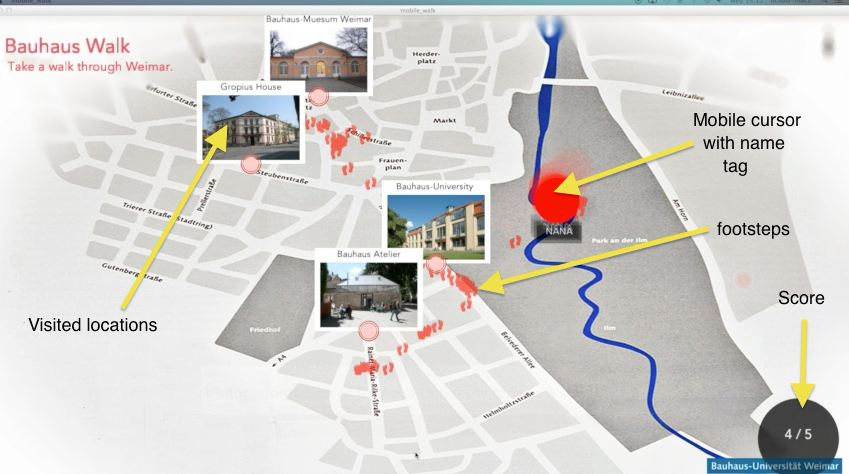
\includegraphics[width=120mm,height=70mm]{Figures/6/mobile/interaction_inter}
    \caption{Mobile interactive interface}%
    \label{fig:mobile_secondinterface}%
\end{figure}



\item Mobile interface: \\
After opening the web page in smartphone, and entering name, the below interface would appear. The interface is very simply designed and has two elements, the cursor and the select button, with cursor the user can navigate inside the map for interest points and when reached on an interest point the participant presses the select button to explore that location, see the picture below.

\hilight{ Florian Echtler's student projects! }

\begin{figure}[H]
    \centering
    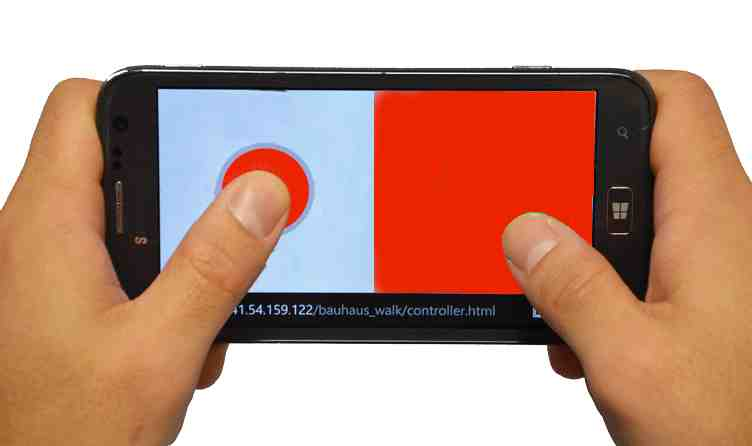
\includegraphics[width=100mm,height=60mm]{Figures/6/mobile/mobile_interface}
    \caption{Mobile controller interface: The left side is the cursor and the right side is the select button.}%
    \label{fig:mobile_controllerinterface}%
\end{figure}


\end{enumerate}

\section{Research questions}

\begin{enumerate}
\item	How fast do users understand call-to-action?
\item	How fast participants react to the call-to-action?
\item	How easy participants understand the interaction task?
\item	How long participants take to finish the interaction or visit all target locations?
\item	What are the major usability flaws that prevent users from advertisement interactions?
\item	What is the difference between mobile and body performance.
\item   How the applications would perform in single user interaction and in multi user interaction?
\end{enumerate}

\subsection{Video advertisement}
\begin{enumerate}
\item	Do participants understand about the content of advertisement?
\item	How many elements of display can participants recall after their first interaction?
\end{enumerate}


\section{Test Design}
This study used a within subject design, in which each participants were asked to experience with both body and mobile interactions, the interaction sequence was interchanged for participants in order to counterbalance the learning effect.


\subsection {Participants}
12 participants were invited for the usability testing; from which five participants were female and seven were male, most of the participants had computer science background and were familiar with mobile and had seen or worked with body sensing technologies, one participant was not familiar with QR-code.

\subsection{Task}
Participants were not told about any specific task, they were told to explore the system by their own and understand what to do, to avoid different outcomes participants were told to continue interaction until they encounter the very first stage of the application. So the tasks for participants were to start from initial stage of the interaction (body /mobile) and continue until reach the initial stage again.

As for body interaction no extra device was required to accomplish the task, but for mobile interaction a mobile phone was required, participants were not told that the use of mobile is required unless participants used their own phone or asked for it from me.

\begin{itemize}

\item Task understandability: \\
Participants were told to think-aloud that what task will they perform at each stage. 


\item Performance measurment: \\

\begin{itemize}
\item call-to-action undrestanding duration \\
The time from when the user saw his/her silhouette until he/she understood / approached to start the interaction. For body call-to-action, if the person intentionally moved toward the screen and for mobile call-to-action, when the person pulled the phone out.

\item Triggering game duration\\
This time is measured from the time the user understood that how to start the interaction, until the user actually starts the interaction. for example in case of mobile interaction, the time is measured from the time the user takes out the mobile until he logins and opens the interaction controller.

\item Task undrestanding duration \\
This time is measured when the users starts the game until he/she undrestands what to do. or how to explore locations.

\item Task completion duration \\
Task completion time is measured from the time interaction starts until the interaction ends. 

\end{itemize}


\item Content recall: \\
After the first interaction with the advertisement, immediately participants were given paper and pen to write down the name of anything that they could recall. The interactions (mobile and body) were counterbalanced between the participants.


\item Usability issues: \\
Each participant was given five minutes to interact with advertisement for both mobile and body and then follow up questions were asked regarding the issues they faced.
The usability issues like (confusing, unclear events and mistakes) were all observed by the moderator at the scene and later while watching the recorded videos. To understand better each interaction was separately listed as below.

\end{itemize}

\subsection{Data Gathering }
The below data were gathered.

\subsection{Performance data}
Check for performance measurements, which were discussed in the previous sections. Each individual's performance with both mobile and body interactions were created in bar chart, this data could also be used to check for efficiency of the interactions techniques too, then to get an overview of performance in general the mean duration of the performance data were computed.


\subsubsection{Preference data}
The preference data, which is the measures of participant opinion or thought process, like the think-aloud each participant performed, or the answers for the interviews and their feedbacks.
\begin{itemize}

\item Think aloud quotes \\
Think-Aloud quotes were noted during the video observation, these quotes were important to check at which point in time users understand about the interaction and tasks. It also helped to analyze their reaction and feedbacks toward the tasks being done.

\item Interview transcripts \\
All the interviews were transcribed and color-coding technique was applied to analyze and comprehend different aspects and categories from the defined questions.


\item Recordings \\
There were two different recordings done during the session, first was video recording using camera at the backside that could record user actions and computer screen, the second recording was the screen recording of the application using QuickTime screen recorder. These recordings were used to analyze behavior, application performance and listen to the things participants said during interaction.


\begin{figure}[H]
    \centering
    \begin{subfigure}[H]{0.45\textwidth}
        \centering
        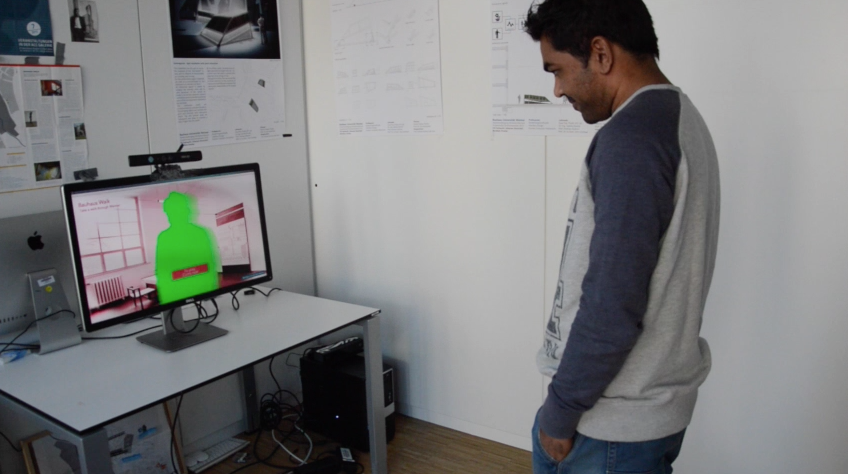
\includegraphics[width=\textwidth,height=4cm]{Figures/6/singleBody}
        \caption{Participant in body interaction mode.}
        \label{fig:singlebody}
    \end{subfigure}
    \begin{subfigure}[H]{0.45\textwidth}
        \centering
        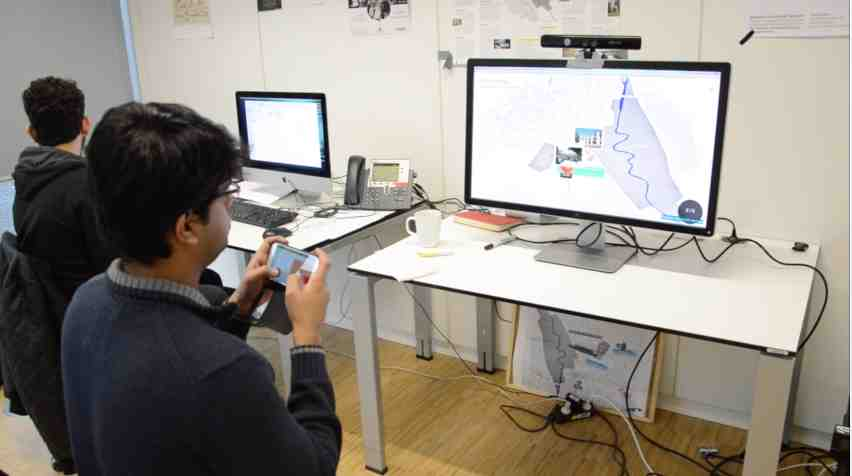
\includegraphics[width=\textwidth,height=4cm]{Figures/6/singleMobile}
        \caption{Participant in mobile interaction mode}
        \label{fig:singleMobile}
    \end{subfigure}
    \caption{Participant's video recordings}
    \label{fig:Focus_group_room}
\end{figure}

\end{itemize}



\section{Findings}


\subsection{User performance}


\begin{itemize}

\item Mobile Interaction performance: \\
The below chart shows the performance data when the mobile interaction happened for participants. The y-axis shows duration in seconds and x-axis shows the aspects as below. You can see performance chart for each individual of body in Appendix \ref{app:body_performance} and of mobile in Appendix \ref{app:mobile_performance}

\begin{figure}[H]
\centering
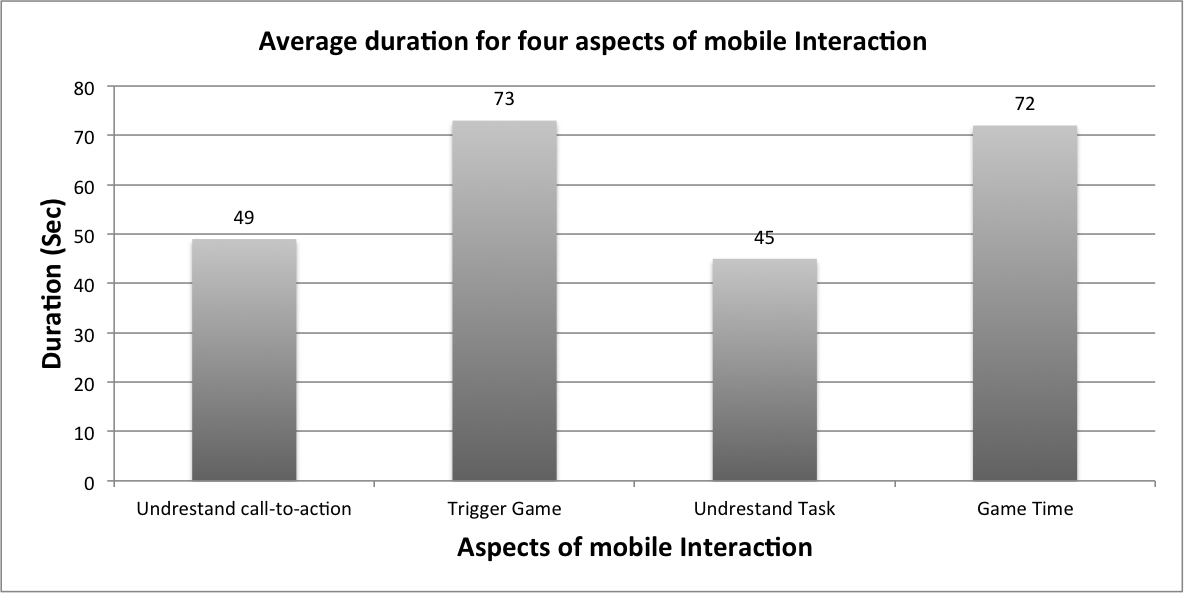
\includegraphics[width=12cm,height=5cm]{Figures/6/mobile_average}%
 \caption{Chart that shows each aspect with respect to duration. }%
 \label{fig:mobile_average}%
\end{figure}

 Participants took 49 seconds in average to understand how to access the system (call-to-action), After participants understood what to do it took 73 seconds in average from taking their phone, opening the web page, logging and starting the game, it took 45 seconds in average to figure out how to do the task and 72 seconds to complete the task, as a result in average 240 seconds were taken for whole interaction time.

%
%\begin{figure}[H]
%\centering
%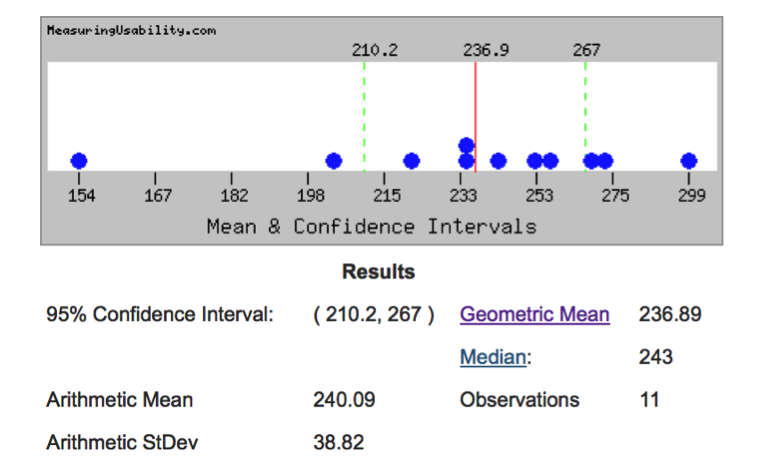
\includegraphics[width=12cm,height=6cm]{Figures/6/mobile_mean}%
% \caption{Confidence interval for Mobile interaction all phases duration }%
% \label{fig:mobile_mean}%
%\end{figure}

%above chart is generated in an online tool [1] with a confidence interval up to 95\% for complete interaction time for all 11 participants; the confidence interval is between (210.2, 267) the chart shows the Arithmetic standard deviation to be up to 38.82 seconds, Arithmetic Mean to be 240 seconds

\item Body Interaction performance: \\
This also shows four different aspects of the body interaction in the below chart.

\begin{figure}[H]
\centering
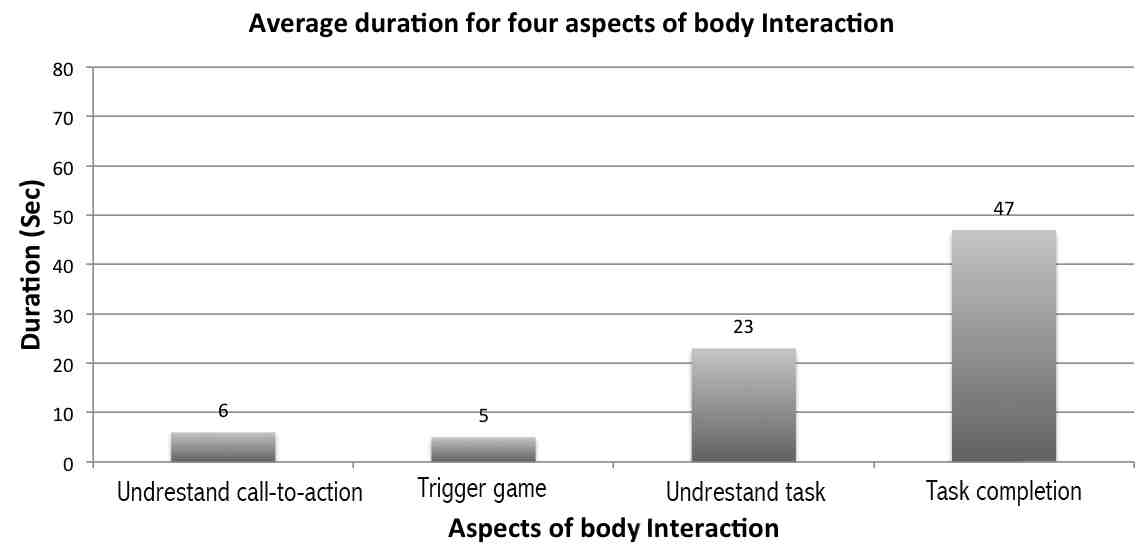
\includegraphics[width=12cm,height=5cm]{Figures/6/body_average}%
 \caption{Chart that shows each aspect with respect to duration}%
 \label{fig:body_average}%
\end{figure}

As can be seen above most of the participants finished the whole interaction in approximately 81 seconds, which is much better than mobile interaction. It took 6 seconds to understand call-to-action, 5 seconds to trigger and start the game, 23 seconds to understand the task and 47 seconds to complete the tasks.

%\begin{figure}[H]
%\centering
%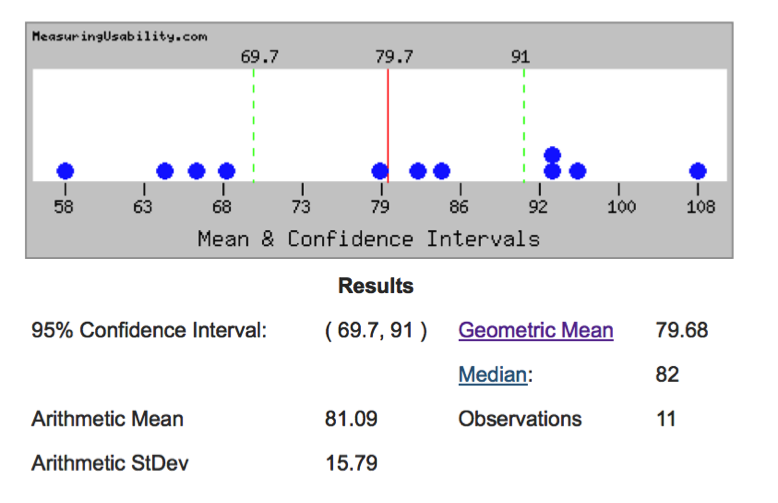
\includegraphics[width=12cm,height=6cm]{Figures/6/body_mean}%
% \caption{Confidence interval for body interaction all phases duration }%
% \label{fig:body_mean}%
%\end{figure}

%The above confidence interval for body interaction is generated using the web tool [1] for whole body interaction time. In which with the confidence interval of 95\% is between (69.7 ? 91) seconds, with the standard deviation of 15.79 seconds.


\item Body Vs. Mobile performance: \\
As can be seen below body interaction seems to be much better than mobile interaction in terms of performance. The whole interaction time of body is less than the half of the time of mobile interaction. 

\begin{figure}[H]
\centering
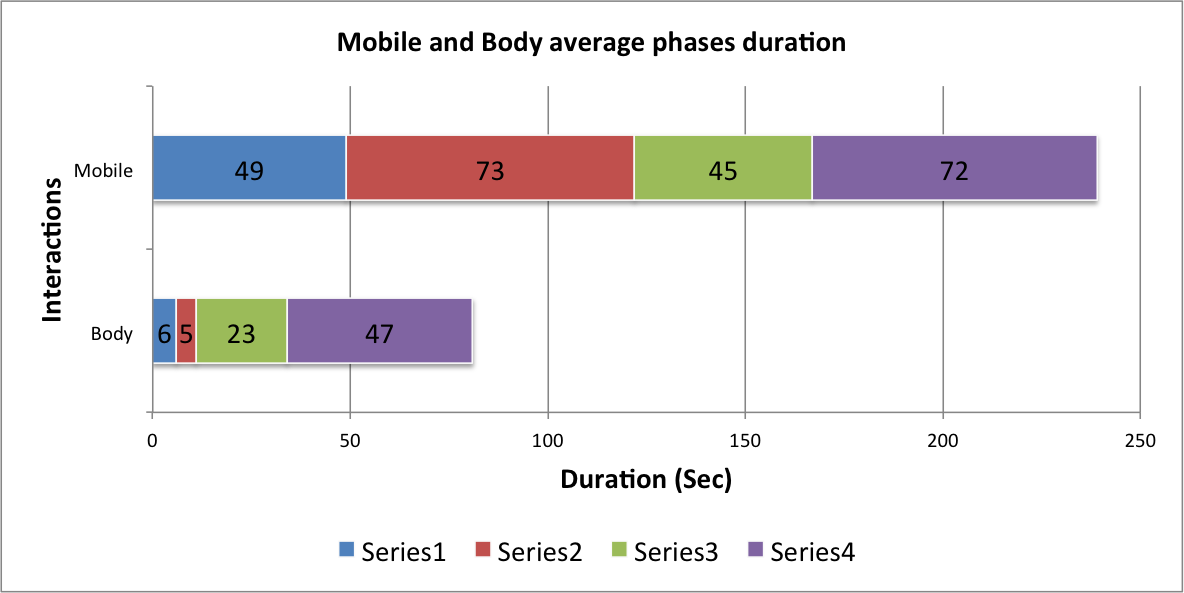
\includegraphics[width=12cm,height=6cm]{Figures/6/mobile_body_performance}%
 \caption{Comparison of body and mobile interaction performance }%
 \label{fig:mobile_body_performance}%
\end{figure}

81 second is the mean value of the all participants with body interaction and 240 seconds is the mean value of the same participants with mobile interaction. The below chart shows other comparison of aspects as described.

\begin{figure}[H]
\centering
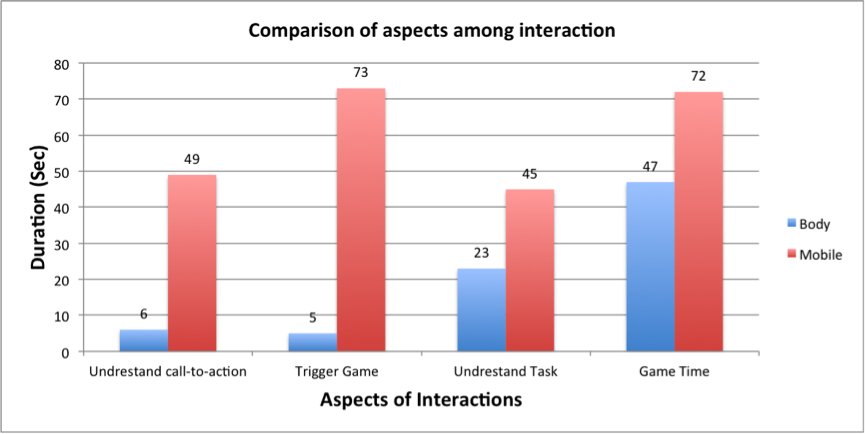
\includegraphics[width=12cm,height=6cm]{Figures/6/mobile_body_aspect}%
 \caption{Comparison of the aspects of interaction among body and mobile }%
 \label{fig:mobile_body_aspect}%
\end{figure}


As can be seen in the chart mobile interaction took much longer than body interaction for each phase or aspects, ANOVA reveals a significant effect of call-to-action of (body vs. mobile)( \emph{(F1,11)=22.4758, p < .001 (p=.0001)}). A post-hoc tukey test shows that participants understood very quickly the call-to-action of body interaction compared to mobile interaction technique, maybe because it is very easy and understandable by any person because of the action ``\emph{to play come near}''is very usual and easy compared to using mobile phone, which is not expected at that moment and the users should read and see the information text to understand, all those steps requires more cognitive load than simple action of body interaction.

ANOVA reveals a significant difference of triggering game between (body vs. mobile) ( \emph{(F1,11)=124.1066, p < .001}). post-hoc tukey test shows that in body interaction the triggering happens much faster than mobile interaction, This is because mobile technique has many steps to follow in order to trigger the game (like connecting to WiFi, logging to website).


ANOVA reveals a significant difference of task undrestandability between (body vs. mobile) ( \emph{(F1,11)=7.1340, p < .05 (p=.0147)}). A post-hoc tukey test shows that participants undrestand the task very faster compared to mobile technique, one hint could be the body representation itself and in mobile an abstract circle is shown and the interface that takes time to try and error and find what to do.

Interaction time is also significantly different as ANOVA test suggests a significant difference between the game interaction ( \emph{(F1,11)=19.7000, p < .001 (p=.01)}) post-hoc tukey test also strongly recommends that body interaction takes less time to complete the interaction comparted to mobile.



\end{itemize}



\subsection{Usability issues}
The below usability issues are gathered from participant while observing them during the interactions.


\begin{itemize}

\item Mobile Interaction: \\


\begin{enumerate}
\item	Call-to-Action
\begin{enumerate}
\item	At the first glance and moment most participants did not try to read the text on the screen, despite they were expecting other way to get quick information, but after many try with their body they had to read the information text. This could be because of many issues like (amount of text, text size and used icons). And most importantly the text information was being covered by the silhouette, if participants were far the text was readable but when participants would get near to the screen to scan the QR-code or read the IP address, the silhouette drawn by the Kinect camera would occlude part of the information text, which resulted that participants should move a side to scan while facing toward the screen.
\item	Participants did not understand about the phone icon or the browser animation on top of it until they figured by themselves.
\item	Frustration of typing the IP address.
\item	The size of QR code was small.
\end{enumerate}

\item	Use of mobile phone.
\begin{enumerate}
\item	Participants did not expect at the beginning that they would use their own phone for the interactions; many times participants asked, ``\emph{Should I use my phone?}'' 
\item	Most participants did not read the instruction to tilt their phone and even if they accidently had tilted the phone, it would have not effected because by default the tilt-sensor of the phones were off because of power saving settings. 
\item	There was no instruction to turn-on the tilt-sensor in mobile phone.
\end{enumerate}

\item	Login page
\begin{enumerate}
\item	Some of the participants were confused with the word Login, Participants thought that they would have to provide some sort of username and password to the system, and one participant reacted to this strictly and refused to login to the webpage using his phone.
\end{enumerate}

\item	Task description
\begin{enumerate}
\item	The task description was shown after the participants login to the system despite of whether the phone is tilted or not, Most participants missed to read the task description because they were busy with their phone to tilt it and by that time the description on the screen was gone.
\end{enumerate}

\item	Controller
\begin{enumerate}
\item	Participants did not read and saw the instructions for phone.	
\item	Many participants complained about the elasticity (automatic centering feature) of cursor. They had to reposition the cursor for another location to explore.
\end{enumerate}
\end{enumerate}



\item Body Interaction: \\

\begin{enumerate}
\item	Call-To-Action \\
The silhouette is projected in the largest scale for attraction attention, but the silhouette scales down (mini-silhouette) and adjusts to person position (x, z) on the display, when users triggered the interaction by coming close to the screen, then participants could not see themselves, because the mini-silhouette would adjust outside at top of the display, if participant moved back then they could see the silhouette back. 

\item	Silhouette controlle \\
There was no instruction on how to move the body physically to perform the tasks, but participants tried themselves to find a way to interact.

\item	Alert image \\
Alert image that shows a Hands-Up person lead to confusion at the moment where users were much closer to the system.
\end{enumerate}

\item Advertisement video: \\
\begin{enumerate}
\item The slides were switching fast.
\item Some did not liked the colors and theme. 
\end{enumerate}


\end{itemize}

\subsection{Advertisement goal}


\begin{itemize}


\item Did users understand about advertisement? \\

	The criteria for recalling the advertisement was that participants should recall ``\emph{Bauhaus-Walk}'' word and explain what does it do or if the interaction technique gave them an idea what could be the advertisement about, At best users can recall the date, timing and location of the tour program.

\begin{enumerate}

\item	\textbf{Ad goal description} \\
Therefor to find out this, when all participants experienced with the very first interaction technique mobile or body, they were immediately asked about the goal of advertisement, we wanted to know if the participants would understand about the advertisement at their very first try. All of the participants were speaking in English language and the advertisement interaction and the entire participants responded as they finished the interaction. 9 participants accurately described the goal of the advertisement and 2 participants generally described about the goal, the reason behind that was advertisement video, which was shown was in German language, later the video was changed to English for the rest of participants and they responded precisely.

\item	\textbf{Ad-related elements recalled}  \\ 
After the participants described the goal, they were given a piece of sheet to draw and write any element related to the interaction and advertisement with in five minutes. All the sketches drawn and keywords written by the participants were manually analyzed and counted

\begin{figure}[H]
\centering
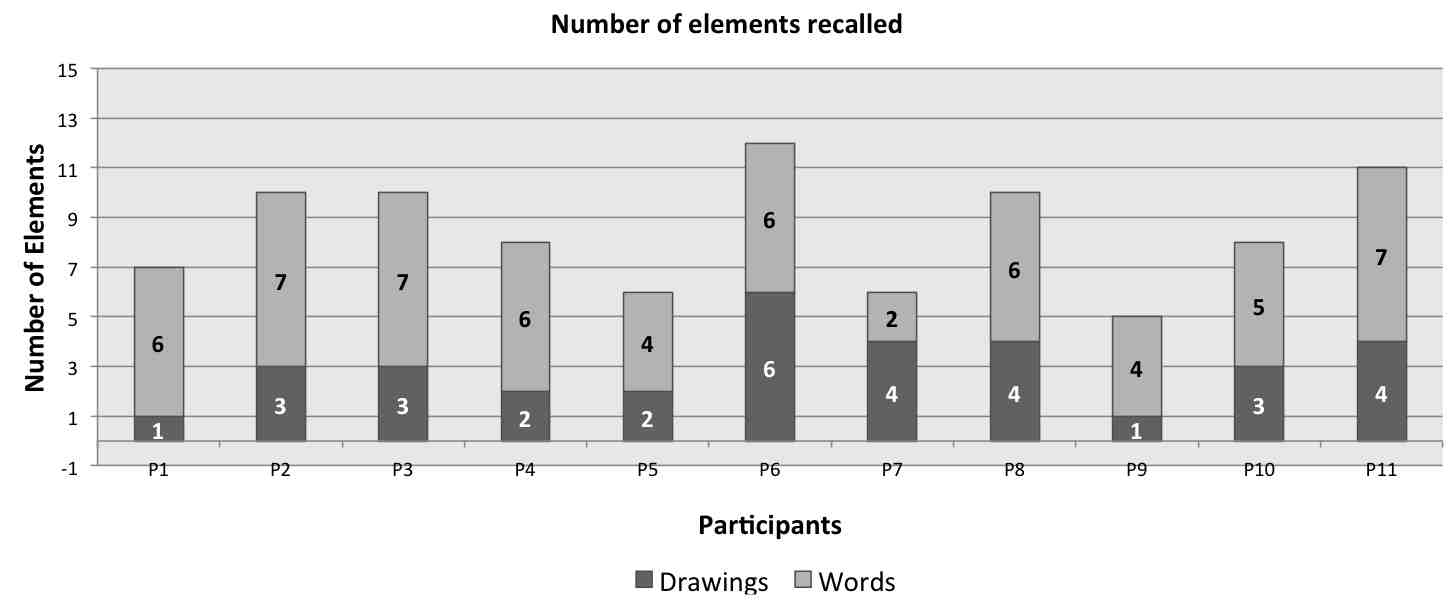
\includegraphics[width=12cm,height=6cm]{Figures/6/word_recall}%
 \caption{Number of words and drawings of the advertisement elements }%
 \label{fig:word_recall}%
\end{figure}

\end{enumerate}

\item Word cloud (Wordle): \\
All the keywords written in the papers by participants were collected in one text file and visualized in world cloude technique by using an online tool\footnote{Wordle: \url{http://www.wordle.net/create}, last accessed: 10 May 2016} the below word cloud was generated.

\begin{figure}[H]
\centering
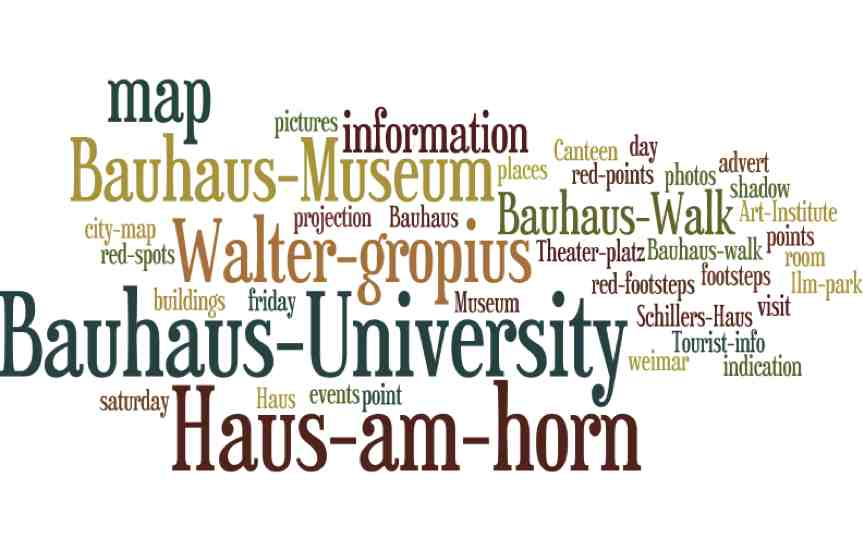
\includegraphics[width=12cm,height=8cm]{Figures/6/wordle}%
 \caption{Word cloud representation of the keywords}%
 \label{fig:wordle}%
\end{figure}

As can be seen, most key words that has high frequency are the ones actually related to the advertisement it seems most location names that participants interacted with are recalled a lot like ``\emph{Bauhaus University}'' ,``\emph{Haus-am-horn}''and others, The program name ``\emph{Bauhaus-Walk}'' is also in high frequency, and even the day of the event is mentioned too.


\item Key factors for advertisement understanding: \\
\begin{enumerate}
\item	\textbf{Game environment} \\
The game environment designed for the interactions had a major impact for understanding the advertisement goal, for example one of the participants replied ``\emph{I saw a map and different places, so I guess touristic places that I can visit in Weimar.}'' Beside the map the blinking points on the map, which more people are familiar that shows interest regions of a city, one participant replied ``\emph{ I think it was about tourist places in the city, at first I saw the map, and there were points on the top}'' By analyzing their reply, they already linked the points with the touristic places.

\item	\textbf{Interaction technique} \\
The interaction technique especially with the body interaction where walking is involved, participants got clue about the advertisement indirectly only by walking and linked walking as visiting locations, like one of the participants replied ``\emph{Discovering Weimar. The Bauhaus-Walk. It was the advertisement about those locations that the people can visit in the tour.}'' It is very fascinating to read that answer from which the whole goal of the advertisement can be derived.

\item	\textbf{Advertisement video} \\
The advertisement video had an impact on the participants to be able to recall the advertisement, one of the participants replied that ``\emph{I saw many pictures coming about Bauhaus and the program times and day}'', despite that the users understood a little about the advertisement they also complained about the video for being fast.

\end{enumerate}

\end{itemize}

\subsection{Interview Findings}
All the interviews transcripts were coded for better analyzing, appropriate connections to categories were found and these categories are shown as a diagram.

\begin{itemize}

\item Mobile Categories: \\
Many important categories were created from the responder's codes, see Appendix \ref{app:mobileinterviewcodes_} for the diagram. These categories reflect the functionality, nature, issues and complications of mobile interaction technique. Most of them points out negative concerns and some positive feedbacks too about the interactions, which is discussed below.
\begin{enumerate}
\item	\textbf{Comfortable} \\
	Mobile interaction is comfortable in the context of public environment, users do not feel shy to work with their phone, they have more privacy as one user said ``\emph{I think for people moving in public could be more embarrassing if you just use your phone the people passing by will not pay attention}''. Users can also work with the display from a far location rather than standing in front as one participant said, ``\emph{you can comfortably set far away see the screen and start interacting}''.
\item	\textbf{Activity} \\
	This method has less Activity, participants do not have to move their body to reach certain points in the map, instead they can use their phone and stand or sit steady and with the tip of their finger can easily explore locations, as one of the user said ``\emph{I could go with the tip of my finger and it helped me all the places I visited}''.
\item	\textbf{Dependency}\\
	On the other hand, this interaction is dependent to many things like obviously a mobile phone, if the user does not have a mobile phone the interaction cannot happen, a participant asked, ``\emph{How would I have played if I have not brought my mobile phone?}'' Another dependency is the WIFI connection, one participant pointed out ``\emph{And then the fact that I had to be connected to a WIFI, that was because I did not understand do we have to be in the same Internet (Network)?}'' 

\item	\textbf{Complicated}\\
The process seemed also complicated like first entering the IP-Address or scanning the QR-code, then looking at the instructions and logging with a name, then tilting the phone and finally interacting with the controller elements like the button and cursor, most of the participants complained about this stating like, ``\emph{Because it is a headache for me to take out my phone and use all this login, and waste my time.}'' another commented like ``\emph{for exploring you have to push that red button, that was a bit confusing.}''


\item	\textbf{Annoying}\\
One of the annoying things pointed out by the participant was the QR-Code was being covered by the person silhouette standing in front of the display the user said ``\emph{QR-Code was small and when I was coming near the screen to scan the code, my body was covering it}''.

\item	\textbf{Clarity}\\
There were many instructions like Access-information, mobile instruction and task instruction, but these instruction was also not clear to them as one of the participant mentioned, ``\emph{that controller was also not clear, because I though the red areas is the touch area that I can scroll and the red button was a click}'' another participant replied like ``\emph{there were very few descriptions, I guess the word login was miss-phrased, it was not really a login it was just chose a name}''. Another participant was not sure if to use mobile phone or the screen has touch capability as he replied ``\emph{at first I saw the map, and there were points on the top first I tried to touch}''.


\end{enumerate}


\item Body Categories: \\
Body interaction was more appreciated by the participants; From the interview transcripts an intensive color code categories were derived, see Appendix \ref{app:bodyinterviewcodes_} for the code diagram. The below positive and negative opinions were derived and categorized. 

\begin{enumerate}
\item	\textbf{Enjoyment}\\
Participants had the sense of enjoyment and fun, as one of participants said, ``\emph{I liked the second one because it seemed more involving and I think it was more fun}'', another user said ``\emph{I liked this interaction; it was more good and fun.}'' , 

\item	\textbf{Easy}\\
Users found the interaction to be very easy, simple and smooth, a user said, ``\emph{The body movement was good it was smooth}'' another user said, ``\emph{It was much easier than the previous one, it was much better, umm it was not confusing}''. The call-to-Action seemed much easier, one user said, ``\emph{I saw saying me to come near, and when I came the game started, that was very easy to use}'', and the interaction with the game elements was also easy to understand, one participants said ``\emph{it was easy to come near to the screen and first I did not understand how to play the game but when I saw my avatar that is moving with me then I realized and did the tasks}''

\item	\textbf{Immersion}\\
Some participants said they were some how immersed with the game, like one said, ``\emph{I felt that I was really part of it}'', another said, ``\emph{With the body you look your own avatar in the map and you feel that you are in the map.}''

\item	\textbf{Engaging}\\
The body technique seemed also very engaging and users wanted to play more and more, one said, ``\emph{It is so engaging and it is like that it needs you}'', another said, ``\emph{it is like you want to put the footsteps exactly on the street}'' , ``\emph{it seemed more involving}''. 

\item	\textbf{Issues}\\
On the other hand, body interaction had also some issues, like one of the participants pointed out that the interaction would be difficult if it is in crowded area, one said, ``\emph{If two people interact then they can crash at each other}''. Participants complained about physical space ``\emph{I felt was the space there was not enough space in here}''. Bad tracking of the body and unexpected locations were triggered by fast movement like, one participants said, ``\emph{I guess the application was tracking me really bad}'', ``\emph{when I was moving to some areas fast suddenly that point was being triggered.}''

\item	\textbf{Embarrassing}\\
Some participants said that they would not try at public because it could be shame or embarrassment for their selves, ?moving in public could be more embarrassing?

\item	\textbf{Confusion}\\
The projection of silhouette on the advertisement also made some participants confused and that was also distractive, like one said, ``\emph{I saw my silhouette at the last time I was playing, because I was curious that why is it there}''. 

\end{enumerate}


\item Others: \\

\begin{enumerate}
\item	\textbf{Interface}\\
The interface was appreciated by all the participants, as one said, ``\emph{I really liked the map}'', another user said, ``\emph{the footsteps were cute}''.

\item	\textbf{Non-controllability}\\
The flow of the interaction was also observed by the users, which they found annoying like, one participants noticed that ``\emph{I do not want to be forced to see all the places and then see the advertisement}'', the video advertisement was also not in the control a user said, ``\emph{There was nothing to answer, it gave me the impression that okay; this was an advertisement someone did it and I could not change the flow of it.}'' 

\item	\textbf{Distraction}\\
The projection of silhouette after the interaction body or mobile technique was a distraction factor, because participants would not notice the video advertisement but would notice themselves. 

\item	\textbf{Speed}\\
The pictures for the locations and the advertisement video were fast, a user said, ``\emph{The description of the places were very fast, when I was trying to read it, it disappeared.}'', 
\end{enumerate}

\end{itemize}


\subsection{Application Performance}
Application performed quite well for both single and multi-user interactions, it did not crashed nor hanged in the middle of interaction, but in multi-user interaction, application faced some delay in both body and mobile because of many participants 5-7 at the same time, this issue got solved by changing the JRE version from 32bit to 64bit and along with this the processing version was also changed from 32bit to 64bit and increased the maximum usage memory to highest in processing.

\hilight{Maybe put some system specifications that run the applications}

\begin{figure}[H]
    \centering
    \begin{subfigure}[H]{0.45\textwidth}
        \centering
        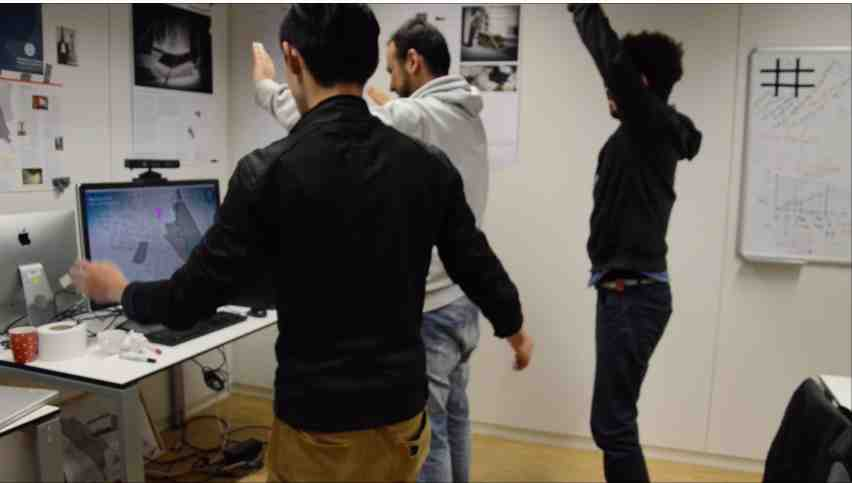
\includegraphics[width=\textwidth,height=4cm]{Figures/6/groupBody}
        \caption{Group body interaction.}
        \label{fig:groupbody}
    \end{subfigure}
    \begin{subfigure}[H]{0.45\textwidth}
        \centering
        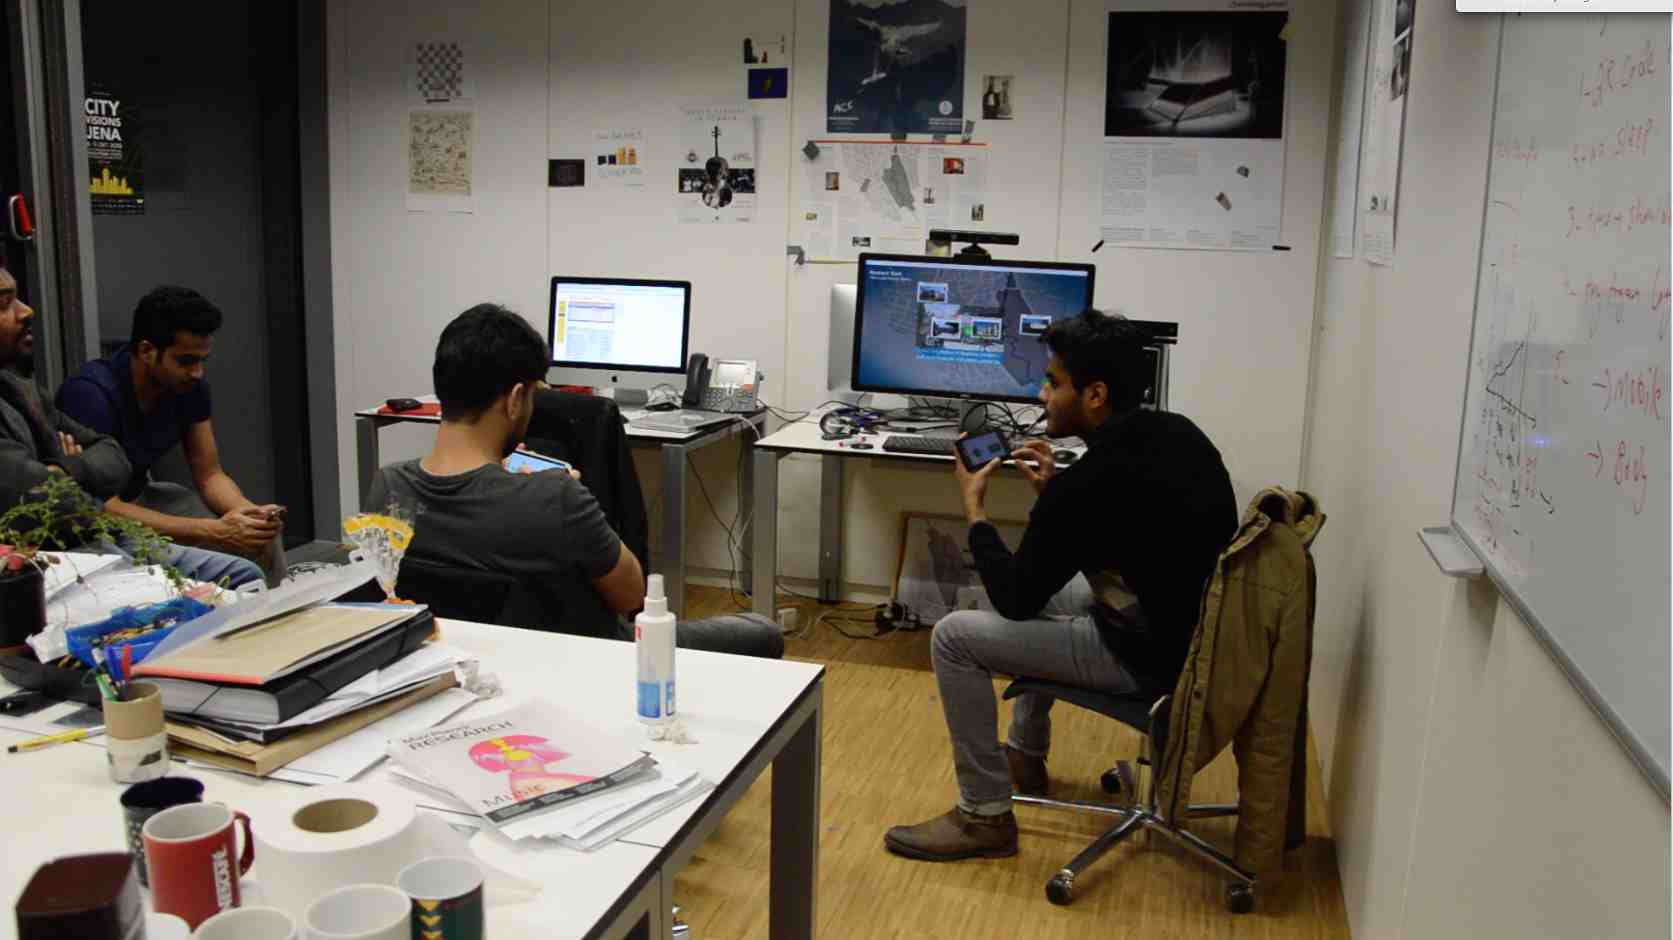
\includegraphics[width=\textwidth,height=4cm]{Figures/6/groupMobile}
        \caption{Group mobile interaction.}
        \label{fig:groupmobile}
    \end{subfigure}
    \caption{}
    \label{fig:Focus_group_room_interactive}
\end{figure}

\newpage
\section{Conclusion}
This chapter concludes that with body interaction technique, users performed better than mobile technique and preferred the use of body interaction than mobile in public environment, but at the same time mobile interaction was also preferred by some participant. 

Body interaction was more natural and convenient for participants. This interaction had no dependency to any preferable device like mobile phone, the call-to-action was very understandable and performing this call-to-action (come near), was very natural. Body representation on the map provided a strong clue of ``\emph{walking}'', this clue had two major benefits, (1) understanding the task and performing it, (2) understanding the goal of the interactive advertisement. Participant felt enjoyment, immersion while interacting using their body. Despite the positive feedbacks, there were some usability issues like incorrect mapping of the silhouette when user was standing near, and some alert messages were not implemented, and also the interaction was difficult if there were multi-user because the users were colliding to each other, but the overall performance and acceptability of this technique was very convincing compared to mobile interaction.

Mobile interaction had various usability issues and especially with the accessibility to the advertisement system, participants took very long time to understand what was required to access because of (unclear access-info text, unfamiliarity with QR code or phone icons, inserting name), and then took longer time to follow the steps to login to the system. Task completion time was also significantly low than body interaction.  Beside all these major issues some participants found it more comfortable to use it in public display because it will not cause the sense of embarrassment for them, and while interaction it did not require more physical body movement but only required cursor movement, and also participants understood the goal of advertisement.

Considering the above issues, the next step would be to refine both prototypes and make it ready for evaluation on public space.














